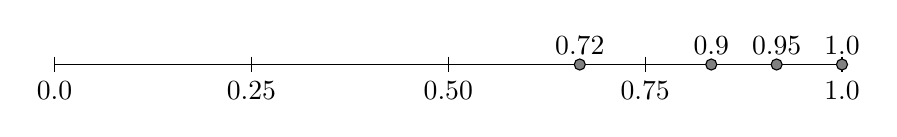
\begin{tikzpicture}
    % Draw number line
    \draw[-] (0,0) -- (10,0) node[right] {};

    % Beschriftung der Hauptmarkierungen
    \foreach \x in {0.0, 0.25, 0.50, 0.75, 1.0} {
        \draw (\x*10,0.1) -- (\x*10,-0.1) node[below] {\x};
    }

    % Die Punkte plotten
    \draw[fill=gray] (0.667*10,0) circle (2pt) node[above] {$0.72$};
    \draw[fill=gray] (0.834*10,0) circle (2pt) node[above] {$0.9$};
    \draw[fill=gray] (0.917*10,0) circle (2pt) node[above] {$0.95$};
    \draw[fill=gray] (1.000*10,0) circle (2pt) node[above] {$1.0$};
\end{tikzpicture}
